\appendix

\section{Bilder}

\begin{figure}[H]
    \centering
    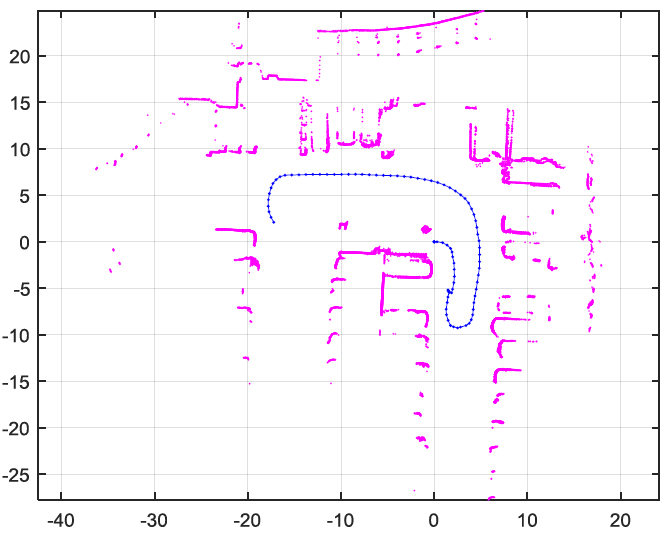
\includegraphics[scale=0.5]{30_Ende/SLAM.png}
\end{figure}
\label{anhang:PNGBILD}
Anhang 1: Beispiel einer Simulation zu Lidar-Slam.

\section{Programme}

\lstinputlisting[language=Matlab]{30_Ende/Strecke.m}
\label{anhang:Matlabcode1}
Anhang 2: MATLAB Programmcode importiert - Regelung einer IT1-Strecke.

\newpage
\begin{lstlisting}[language=Matlab]
%% Std-Regelkreis mit P-Regler
kR = 10;
K = kR % P-Regler
Fo = K*G; % ÜF-offene Schleife
T = Fo/(1+Fo); % Führungs-ÜF
T = minreal(T) % Kürzen
Fst = G/(1+Fo); % Störungs-ÜF
figure(2); step(T); grid on
title('Führungs-Sprung mit P-Regler')
figure(3); step(Fst); grid on;
title('Sprung Störungs-ÜF mit P-Regler');

%% Std-RK mit PI-Regler
kR2 = 10;
TN = 1;
Kpi = kR2*(1+s*TN)/(s*TN)
Fo2 = Kpi*G; % ÜF-offene Schleife
T2 = Fo2/(1+Fo2); % Führungs-ÜF
T2 = minreal(T2); % Kürzen
Fst2 = G/(1+Fo2); % Störungs-ÜF
figure(20); step(T2); grid on
title('Führungs-Sprung mit PI-Regler')
figure(21); step(Fst2); grid on;
title('Sprung Störungs-ÜF mit PI-Regler');
\end{lstlisting}
\label{anhang:Matlabcode2}
Anhang 3: MATLAB Programmcode kopiert - Regelung einer IT1-Strecke.